\documentclass{article}
\usepackage[utf8]{inputenc}
\usepackage{amsmath,amsthm,amssymb}
\usepackage{amsfonts}
\usepackage{arydshln}
\usepackage{enumitem}
\usepackage{float}
\usepackage{graphicx}
\usepackage{hyperref}
\usepackage{listings}
\usepackage{makecell}
\usepackage{mathtools}
\usepackage[margin=0.75in]{geometry}
\usepackage{multicol}
\usepackage{subcaption}
\usepackage{wrapfig}
\allowdisplaybreaks
\newtheorem{theorem}{Theorem}
\newtheorem{lemma}{Lemma}

\usepackage{fancyhdr}
\pagestyle{fancy}
\fancyhf{}
\fancyhead[L]{Bridgette Delight}
\fancyhead[C]{Math 465 - Homework 01}
\fancyhead[R]{\thepage}
\renewcommand{\headrulewidth}{2pt}

\title{{\large Math 465}\\ Homework 01}
\author{Bridgette Delight}
\date{\today}

\begin{document}

\maketitle

\section{}
By following the steps of the proof of Theorem 1.1 and the proof of The Contraction Mapping Theorem, prove the following facts:

\begin{enumerate}[label = (\alph*)]
    \item the function $f(x)= \frac{1}{\sqrt{2}+0.5x}-1.5x$ has exactly one root in the interval $\left[0, \frac{1}{2}  \right]$,
    \item the sequence of approximations $\left\{ s_k \right\}^{\infty}_{k=0}$ defined recursively by 
    \begin{equation}\label{cases}
    \begin{cases}
    s_0 \in \left[0, \frac{1}{2} \right] - \text{arbitrary}\\
    s_{k+1} = \frac{2}{3\sqrt{2}+1.5s_k}, &k=0,1,2,\dots
    \end{cases}
    \end{equation}converges to the root.
\end{enumerate}


\vspace{10mm}

\subsection*{(a)}



\begin{align*}
    \text{To show that $f(x)$ has exactly 1 root, we first have to}&\\
    \text{show that a root exists to begin with. So, if}&\\
    f&:[a,b] \to \mathbb{R} \text{ is continuous and}\\
    [a,b] &= \left[0,\frac{1}{2}\right]\\
    \text{and,}&\\
    0 &\ge f(a) \cdot f(b)\\
    \text{then, }&\\
    &\exists \text{ } \xi \in [a,b] \text{ where, }f(\xi)=0 \\
    f(x)&= \frac{1}{\sqrt{2}+0.5x}-1.5x \text{ for }x \in \left[0,\frac{1}{2}\right] \\
    \text{We will use the intermediate value theorem to prove }&\\
    \text{that there is a 0 between $f(a)$ and $f(b)$ }&\\
    0 &\le f(a) \cdot f(b)\\
    f(a)&=f(1)>0\\
    f(b)&=f\left(\frac{1}{2}\right)<0 \\
    f(x) &= \frac{1}{\sqrt{2}+0.5x}-1.5x\\
    f(0)&= \frac{1}{\sqrt{2}+0}-0\\
    0&< \frac{1}{\sqrt{2}}=f(a)\\
    f\left(\frac{1}{2}\right) &= \frac{1}{\sqrt{2}+\frac{1}{2} \cdot \frac{1}{2}}-\frac{3}{2} \cdot \frac{1}{2}\\
    &= \frac{1}{0.25 + 1.414}-\frac{3}{4}\\
    0&> 0.60088 - .75 =f(b)\\
    \text{Therefore, a root exists in the interval $[a,b]$.}&\\
    \text{In order to show uniqueness we will say that since}&\\
    \text{$f(x)$ has a root, then there exists a}&\\
    g&:g(x)=0\\
    \Rightarrow f(x)&= g(x)-x=0\\
    \text{So,}&\\
    g(x)&= \frac{2}{3\sqrt{2}+1.5x}\\
    |x-y|&= |g(x)-g(y)|\\
    \text{From the Mean Value Theorem we get,}&\\
    |x-y|&\le |g(x)-g(y)|=|g'(z)(x-y)| \text{, while }z \in [x,y]\\
    g'(x) &= \frac{-3}{(3\sqrt{2}+1.5x)^2}\\
    \text{As $g(x)$ is a monotone decreasing function within the}&\\
    \text{bounds of $\left[0, \frac{1}{2}\right]$ we can find the upper bound.}&\\
    g'(0)&= \frac{1}{6}\\
    \Rightarrow |x-y|&= |g(x)-g(y)| \le \frac{x-y}{6}\\
    \text{Therefore $g$ is a contraction.}&\\
    \text{To show that the root is unique we will use a proof}&\\
    \text{by contradiction.}&\\
    \text{We make the assumption that there exists}&\\
    \text{two fixed points $\eta$ and $\xi$. So,}&\\
    |\xi - \eta|&= |g(\xi)-g(\eta)|\le \bigg | \frac{\xi - \eta}{6}\bigg |\\
    \Rightarrow |\xi - \eta|& \le \bigg | \frac{\xi - \eta}{6}\bigg |\\
    \Rightarrow \frac{| \xi - \eta|}{|\xi - \eta|}& \le \frac{1}{6}\\
    \text{Which means, }&\quad 1 \le \frac{1}{6}\\
    \text{Which is wrong. Thus, it is a contradiction meaning}&\\
    \text{that there exists only one fixed point for $g$.}
\end{align*}

\vspace{10mm}
\subsection*{(b)}
% page 14

\begin{align*}
    \text{To show that equation \ref{cases} is a sequence that}&\\
    \text{converges to the root first we prove that,}&\\
     \lim_{k \to \infty} x_k&= \xi, \qquad x_0 \in \left[0, \frac{1}{2} \right]\\ \\
     \lim_{k \to \infty} |x_k - \xi|&= 0\\
     \text{Conjecture:}\\
     P(k) &= |x_k-\xi| \le \left(\frac{1}{6} \right)^k|x_0-\xi| \text{, for }k=0,1,2,\dots\\
     P(0) &= |x_0-\xi| \le \left(\frac{1}{6} \right)^0|x_0-\xi| \\
     \text{So,}&\\
     &|x_0- \xi| \le |x_0 - \xi|\\
     \text{and $P(0)$ is satisfied $P(K) \Rightarrow P(k+1)$}&\\
     \text{for all $k$. In other words}&\\
     &|x_k- \xi|\le \left(\frac{1}{6} \right)^k |x_{k-2}-\xi|\\
     \Rightarrow &|x_{k+1}- \xi| \le  \left(\frac{1}{6} \right)^{k+1} |x_{0}-\xi|\\
     &x_{k+1} = \frac{2}{3\sqrt{2}+1.5\cdot x_k} \\
     &g(x_k) = \frac{\frac{2}{3}}{\sqrt{2}+1.5\cdot x_k}\\
     0 &\le \left(\frac{1}{6} \right)^0 |x_k-\xi|= |g(x_{k-1})-g(\xi)|\\
     & \le \left(\frac{1}{6} \right)^1|x_{k-1}-\xi|= \left(\frac{1}{6} \right)|g(x_{k-2})-g(\xi)| \\
     &\le \left(\frac{1}{6} \right)^2 |x_{k-2}-\xi|\\
     \text{Conjecture:}\\
     P(k) &= |x_k-\xi| \le \left(\frac{1}{6} \right)^k|x_0-\xi| \text{, for }k=0,1,2,\dots\\
     \text{Verify that these conditions are true:}&\\
     1.)&P(k_0)\\
     2.)&P(k) \Rightarrow P(k+1)\text{, for all }k \le k_0\\
     \text{then, $P(k)$for all }k \le k_0\\
     \text{In our example }k_0=0 \text{ that is,}\\
     \text{this condition 1.) is written in the form,}\\
     &|x_0-\xi| \le \left(\frac{1}{6} \right)^k|x_0-\xi|\\
     \text{To prove condition 2.), we assume that,}&\\
     |x_{k}-\xi|&\le \left(\frac{1}{6} \right)^{k}|x_0-\xi|\\
     \text{in order to prove,}\\
     |x_{k+1}-\xi|&\le \left(\frac{1}{6} \right)^{k+1}|x_0-\xi|\\
     \text{So we get,}&\\
     |x_{k}-\xi|&=|g(x_k)-g(\xi)| < \left(\frac{1}{6} \right)|x_k-\xi|\\
     & \le \frac{1}{6}\cdot \left(\frac{1}{6} \right)^k|x_0-\xi|= \left(\frac{1}{6} \right)^{k+1}|x_0-\xi|\\
     \text{By mathematical induction the conjecture}&\\
     P(k) &= |x_k-\xi| \le \left(\frac{1}{6} \right)^k|x_0-\xi| \text{, for }k=0,1,2,\dots\\
     \text{is proved for all $k \ge 0$, }k=0,1,2,\dots &\\
     \text{Since}&\\
     0 & \le |x_k-\xi| \le \left(\frac{1}{6} \right)^{k+1}|x_0-\xi| \text{, for all }k \ge 0\\
     \text{By the squeeze theorem,}&\\
     0&= \lim_{k \to \infty} |x_k - \xi|\\
     \text{because,}\\
     0& =\lim_{k \to \infty} \left(\frac{1}{3} \right)^k\\
     \text{and}&\\
     0& =\lim_{k \to \infty}0\\
     \text{that is,}\\
     \xi &= \lim_{k \to \infty}x_k\\
\end{align*}

% \begin{align*}
%     \text{First, we need to verify that $a$ and $b$}&\\
%     \text{ have different signs.}&\\
%     f_{k+1} &= \frac{2}{3\sqrt{2}+1.5s_k}=g(x_k)\\
%     g(x) &= x \\
%     x &= \frac{2}{3\sqrt{2}+1.5x}\\
%     0 &= \frac{2}{3\sqrt{2}+1.5x}-x\\
%     f(0) &= \frac{2}{3\sqrt{2}+1.5(0)}-0\\
%     &= \frac{2}{3\sqrt{2}} \approx \frac{1}{4}\\
%     f\left(\frac{1}{2}\right) &= \frac{2}{3\sqrt{2}+1.5(\frac{1}{2})}-\frac{1}{2}\\
%     &\approx \frac{1}{4}-\frac{1}{2}=-\frac{1}{4}\\
% \end{align*}


\section{}
Take $s_0 = \frac{1}{\sqrt{6}}$ in (\ref{cases}) and write a code that you can use to compute the first 10000 elements of the sequence $\left\{ s_k \right\}^{\infty}_{k=0}$.
\vspace{10mm}




\begin{table}[H]
    \centering
    \begin{tabular}{|r|c|}
        \Xhline{1 pt}
         \textbf{k}& \textbf{$s_k$}  \\
         \Xhline{1.5 pt}
         0 & 0.4082482904638631\\
         \Xhline{1 pt}
         1 & 0.4119453334948641\\
         \Xhline{1 pt}
         2 & 0.41147533208484804\\
         \Xhline{1 pt}
         3 & 0.4115350233838435\\
         \Xhline{1 pt}
         $\vdots$ & $\vdots$\\
          \Xhline{1 pt}
         9,999 & 0.4115282959774586\\
          \Xhline{1 pt}
         10,000 & 0.4115282959774586\\
         \Xhline{1 pt}
    \end{tabular}
    \caption{Abbreviated table for the sequence $\left\{ s_k\right\}_{k=0}^{10000}$}
    \label{tab:10sequence}
\end{table}


\section{}
Determine a formula for the exact value of the root $\xi \in \left[0,\frac{1}{2} \right]$ of the function $f$.
\vspace{10mm}

\begin{align*}
    f(x) &= \frac{1}{\sqrt{2}+0.5x}-1.5x\\
    0 & = \frac{1}{\sqrt{2}+0.5x}-1.5x\\
    1.5x &= \frac{1}{\sqrt{2}+0.5x}\\
    1 &= 1.5x(\sqrt{2}+0.5x^2)\\
    1 &= 1.5x\cdot \sqrt{2}+ .75x^2\\
    0 &=  .75x^2+ 1.5x\cdot \sqrt{2}-1\\
    \text{Now use the quadratic equation}&\\
    &\frac{-1.5\sqrt{2} \pm \sqrt{(1.5\sqrt{2})^2}-4\cdot.75\cdot -1}{1.5}\\
    \text{Which results in the answer,}&\\
    &\frac{-1.5\sqrt{2}\pm \sqrt{7.5}}{1.5}\\
    0.4115 &\approx \frac{-1.5\sqrt{2}+ \sqrt{7.5}}{1.5}\\
    -3.24 &\approx \frac{-1.5\sqrt{2}- \sqrt{7.5}}{1.5}\\
    \xi &= 0.4115\\
\end{align*}

\section{}
Run your code and present a table that displays the iteration number $k \in {1,2,\dots,15}$ in the first column, the corresponding approximations $s_k$ in the second column, and the corresponding errors of the approximations in the third column.
\vspace{10mm}

\begin{table}[H]
    \centering
    \begin{tabular}{|r|l|c|}
        \Xhline{1 pt}
         \centering \textbf{k}& \textbf{$s_k$}& \textbf{Error}  \\
         \Xhline{1.5 pt}
         0 & 0.4082482904638631&$3.280006\cdot e^{-03}$\\
         \Xhline{1 pt}
         1 & 0.4119453334948641&$4.170375\cdot e^{-04}$\\
         \Xhline{1 pt}
         2 & 0.41147533208484804&$5.296389\cdot e^{-05}$\\
         \Xhline{1 pt}
         3 & 0.4115350233838435&$6.727406\cdot e^{-06}$\\
         \Xhline{1 pt}
         4 & 0.41152744148658515 &$8.544909\cdot e^{-07}$\\
         \Xhline{1 pt}
         5 & 0.41152840451205874 & $1.085346\cdot e^{-07}$\\
          \Xhline{1 pt}
         6 & 0.41152828219175736 & $1.378570\cdot e^{-08}$\\
          \Xhline{1 pt}
         7 & 0.41152829772847227 &$2.224078\cdot e^{-09}$\\
          \Xhline{1 pt}
         8 & 0.41152829575505073 &$2.824962\cdot e^{-10}$\\
          \Xhline{1 pt}
         9 & 0.4115282960057081 &$3.588019\cdot e^{-11}$\\
          \Xhline{1 pt}
         10 & 0.4115282959738705 &$3.588019\cdot e^{-12}$\\
          \Xhline{1 pt}
         11 & 0.41152829597791435 &$4.558576\cdot e^{-13}$\\
          \Xhline{1 pt}
         12 & 0.41152829597740076 &$5.773160\cdot e^{-14}$\\
          \Xhline{1 pt}
         13 & 0.411528295977466 &$7.494005\cdot e^{-15}$\\
          \Xhline{1 pt}
         14 & 0.4115282959774577&$7.771561\cdot e^{-16}$\\
          \Xhline{1 pt}
         15 & 0.41152829597745877&$2.775558\cdot e^{-16}$\\
         \Xhline{1 pt}
    \end{tabular}
    \caption{Values for the sequence$\left\{ s_k\right\}_{k=0}^{15}$}
    \label{tab:15sequence}
\end{table}


\section{}
Present a figure showing the approximations $s_k$ (vertical axis) versus the iteration index $k$ (horizontal axis) for $k=1,2,\dots,15$.
\vspace{10mm}

\begin{figure}[H]
    \centering
    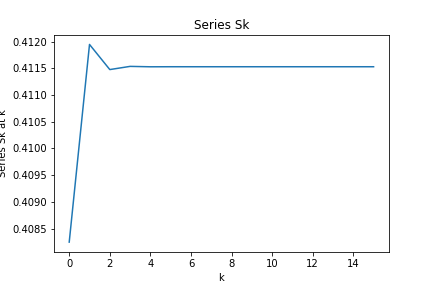
\includegraphics[width = .7\linewidth]{images/hw01q05.png}
    \caption{Figure}
    \label{fig:sk}
\end{figure}


\section{}
Present a figure showing the errors $|s_k - \xi|$ of the approximations (vertical axis) versus the iteration index $k$ (horizontal axis) for $k=1,2,\dots,15$.
\vspace{10mm}

\begin{figure}[H]
    \centering
    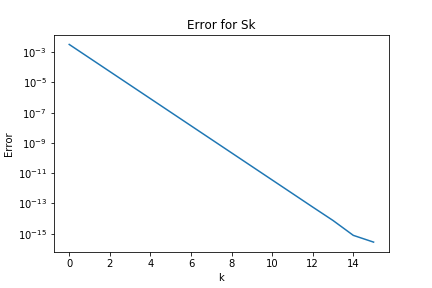
\includegraphics[width = .7\linewidth]{images/hw01q06.png}
    \caption{Graph showing Error at $k$}
    \label{fig:error}
\end{figure}


\section{}
For any $s_0 \in \left[0, \frac{1}{2} \right]$, derive an upper bound on the number of iteration $k$ required to ensure that the $k^{th}$ iterate $s_k$ is correct to six decimal digits. Shows all steps of your derivation. Write down the value of the upper bound in case $s_0 = \frac{1}{\sqrt{6}}$.
\vspace{10mm}

\begin{align*}
    \text{If we assume that:}
    g&:[a,b] \to [a,b] \text{ is continuous}\\
    g&: \text{ is a contraction}\\
    x_0&=\in [a,b]\\
    x_{k+1}&= g(x_k) \text{ for }k=0,1,2, \dots \\
    \text{then,}&\\ 
    \forall& \varepsilon>0 \text{ }\exists k_0(\varepsilon)\in \mathbb{Z}_+ \text{ } \forall k \ge k_0(\varepsilon) |k_k-\xi|\ge \varepsilon\\
    \text{and,}&\\
    k_0(\varepsilon)& \le \left[ \frac{\ln{|x_1-x_0|}-\ln{(\varepsilon(1-L))}} {\ln{\frac{1}{L}}}\right]\\
    \text{where $[x]$ is the floor operation}&\\
    \text{we have}&\\
    |x_k-\xi|& \le L^k|x_0-\xi|\\
    0&=\lim_{k \to \infty}L^k \text{ as }L \in (0,1)\\
    0&=\lim_{k \to \infty}L^k|x_o-\xi|\\
    \forall& \varepsilon>0 \text{, }\exists N \text{, }\forall k \ge N \text{ where }L^k|x_0|\le \varepsilon\text{, and }L^N|x_0|\le \varepsilon\\
    \text{Now we replace $|x_0-\xi|$ with $|x_0-x_1|$ to eliminate $\xi$}\\
    |x_0-\xi| = |x_0-x_1+x_1-\xi| \le |x_0-x_1|&+|x_1-\xi| \le |x_0-x_1| + L|x_0-\xi|\\
    \text{So, }&\\
    |x_0-\xi| \le |x_0-x_1| +L|x_0-\xi| &\Longleftrightarrow{} |x_0-\xi|-L|x_0-\xi| \le|x_0-x_1|(1-L|x_0-\xi|\le |x_0-1|)\\
    &\Rightarrow |x_0-\xi| \le \frac{1}{1-L}|x_0-x_1|\\
    \text{So from  $|x_k-\xi| \le L^k|x_0-\xi|$ ,}&\\
    |x_k-\xi| &\le L^k|x_0-\xi|\le L^k \frac{1}{1-L}|x_0-x_1|\\
    \text{So,}&\\
    |x_k-\xi|& \le \frac{L}{1-L}|x_0-x_1|\\
    \text{Since, $L^k \xrightarrow[k \to \infty]0$,}\\
    0 &=\lim_{k \to \infty}\frac{L}{1-L}|x_0-x_1|\\
    \Longleftrightarrow \forall& \varepsilon>0 \text{ }\exists N\text{ } \forall k \ge N \text{ }|x_k-\xi|\ge \varepsilon\\
    \text{So we define $k_0(\varepsilon)=N$}&\\
    \varepsilon &\ge \frac{L^k}{1-L}|x_0-x_1|\\
    \frac{L^{k+1}}{1-L}|x_0-x_1|&\le \frac{L^k}{1-L}|x_0-x_1| \le \varepsilon\\
    \log(\varepsilon) &\ge \log\left(\frac{L^k}{1-L}|x_0-x_1|  \right)\\
    \log(\varepsilon) &\ge \log(L^k)+\log \left(\frac{|x_0-x_1|}{1-L}  \right)\\
    k &\ge \frac{\log(\varepsilon)-\frac{|x_0-x_1|}{1-L}}{\log(L)}=\frac{\log{\left(\frac{|x_0-x_1|}{1-L}\right)-\log(\varepsilon)}}{\log{\frac{1}{L}}}\\
    &= \frac{\log{(|x_0-x_1|)}-\log{(1-L)}-\log{(\varepsilon)}}{\log{\frac{1}{L}}}\\
    &=\frac{\log{(x_0-x_1)}-\log{(\varepsilon(1-L))}}{\log{\frac{1}{L}}}\\
    &= \alpha\\
    k_0(\varepsilon)&\le \left[\frac{\log{(x_0-x_1)}-\log{(\varepsilon(1-L))}}{\log{\frac{1}{L}}} \right]+1\\
\end{align*}

\begin{align*}
    \varepsilon&=10^{-6}&l&=\frac{1}{6} &x_0 &= \frac{1}{\sqrt{6}}&x_1&= \frac{2}{3\sqrt{2}+1.5(\frac{1}{\sqrt{6}})}=0.41194533349\\
\end{align*}

\begin{align*}
    k_0(10^{-6})&\le \left[ \frac{\log{(\frac{1}{\sqrt{6}}-0.4119453)}-\log{(10^{-6}(1-\frac{1}{6}))}}{\log{\frac{1}{\frac{1}{6}}}} \right]+1\\
     k_0(10^{-6})&\le \left[ \frac{\log{(|-0.003697|)}-\log{(0.0000008\overline{3})}}{\log{(6)}} \right]+1\\
      k_0(10^{-6})&\le [4.68681]+1= 4+1 = 5\\
      \text{It is accurate to 6 decimal digits is when $k=5$.}
\end{align*}


\section{}
Run your code with $s_0 \in \left[0,\frac{1}{\sqrt{6}} \right]$ and find the index $i$ of the first iterate $s_i$ that is correct to six decimal digits. Compare this to your answer to question 7. Is this what you have expected? Why?
\vspace{10mm}

Yes, because when $k=5$ you see in Figure \ref{fig:error}, $k=5$ is where the graph flattens out. It is also the answer from question 7.

\section*{Appendix}

\begin{verbatim}
    def Sk(n):
    sequence = [0, (1/math.sqrt(6))]
    q = 3*math.sqrt(2)
    for index in range(n):
        sequence.append(2/(q+1.5*sequence[-1]))
    return sequence
    
    df = pd.DataFrame(Sk(10000))
    df = df.iloc[1:]
    df = df.reset_index(drop=True)
    
    df = pd.DataFrame(Sk(15))
    df = df.iloc[1:]
    df = df.reset_index(drop=True)
    df = df.reset_index()
    df = df.rename(columns = {0: 'Sk'})
    df['Error'] = df.apply(lambda row : abs(row['Sk']-((-1.5*math.sqrt(2)+
        math.sqrt(7.5))/1.5)), axis = 1) 
    df.to_pickle('sk15.pkl')
    df
    
    
    import matplotlib.pyplot as plt

    df = pd.read_pickle('sk15.pkl')

    plt.plot(df['index'],df['Sk'])
    plt.ylabel('Series Sk at k')
    plt.xlabel('k')
    plt.title('Series Sk')
    plt.savefig('hw01q05.png')
    plt.show()
    
    
    import matplotlib.pyplot as plt

    df = pd.read_pickle('sk15.pkl')

    plt.plot(df['index'],df['Error'])
    plt.ylabel('Error for Sk at k')
    plt.xlabel('k')
    plt.title('Error')
    plt.savefig('hw01q06.png')
    plt.show()
\end{verbatim}


\end{document}